% !TEX root = ../main.tex
\chapter{Overview of the Approach}
\label{chap:overview-of-the-approach}

In this chapter I introduce the high level architecture overview of the proposed framework. Also look at the components one-by-one and discuss how they cooperate, in detail.

\section{Architecture}
\label{sect:architecture}
\Cref{fig:architecture-overview} shows the overview of the framework's architecture. Since the novelty of the approach is how the source code representation is handled --- stored, transformed, and queried --- the heart of the approach is visualized on the right half of the figure. This is embedded and utilized in the framework itself, and integrated into the continuous integration circle and user-facing systems.

\begin{figure}[!htb]
  \centering
  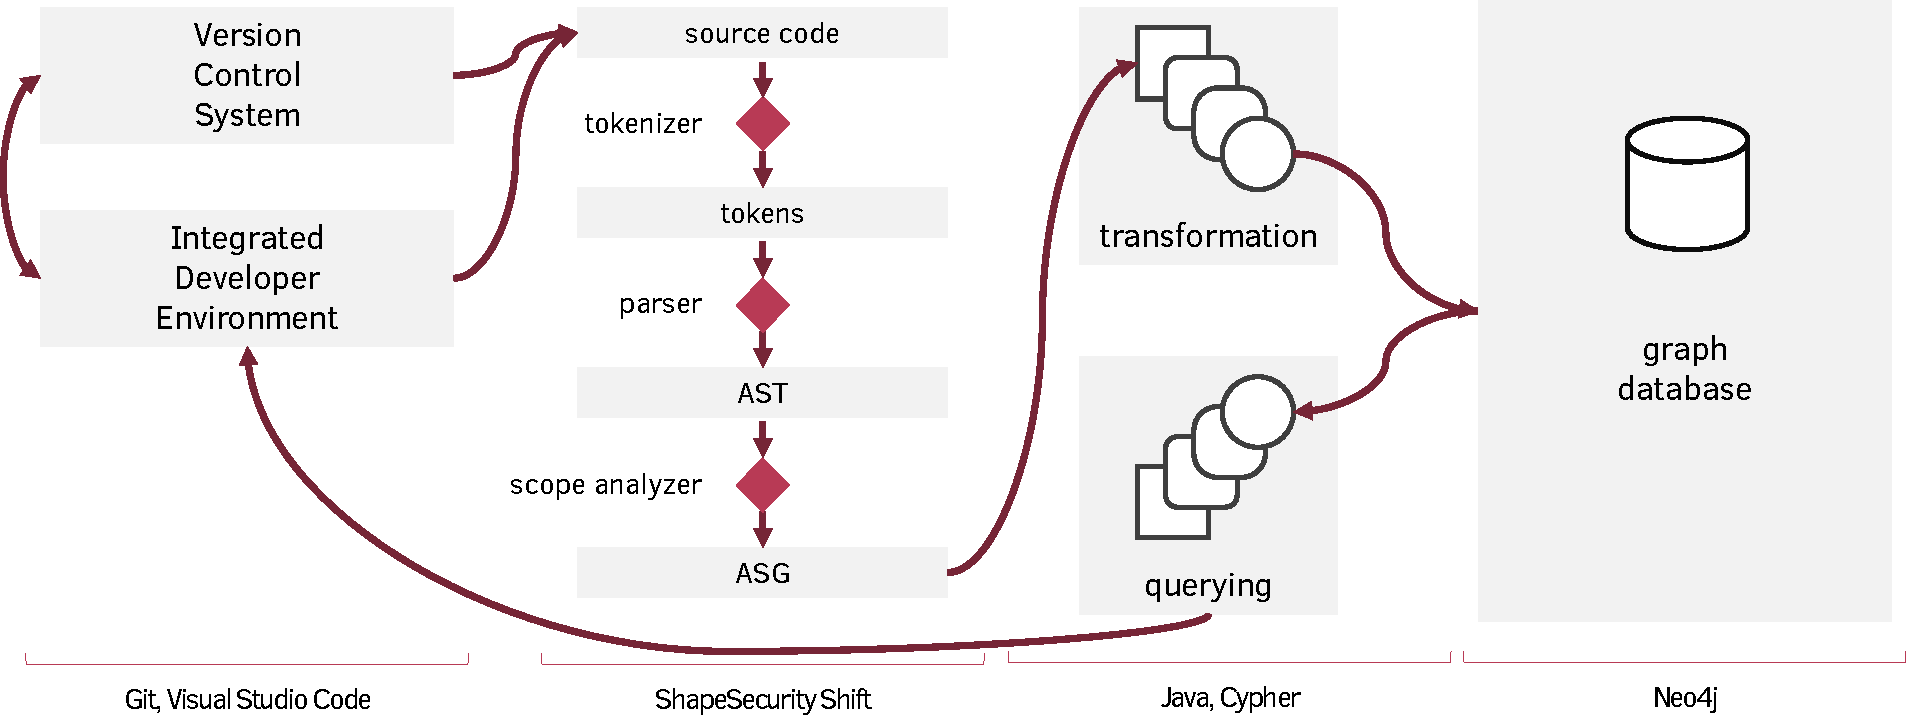
\includegraphics[width=\textwidth]{architecture-PPT.pdf}
  \caption{Architecture Overview of the Approach}
  \label{fig:architecture-overview}
\end{figure}


\section{Main Components}

\subsection{Workflow Integration Points}
The framework is intented to be integrated with at least two types of workflow components. First, connecting to the \emph{Version Control System} makes it possible to extend the continuous integration workflow and provide the users of the system with current information about the codebase they are working on. Second, connecting to the \emph{Integrated Development Environment} of every user empowers them with proactive feedback on their modifications.

\subsubsection{Version Control System (VCS)}
Version control systems are file change (e.g. documents, software code, etc.) management systems. They store revisions of the current set of files managed by the system. Each revision is differentiated with a timestamp, and a person performing the changes are also associated with a revision.

Version control is one of the most essential collaboration tool. When developers work on the same codebase, especially when the codebase is large, they need to share the code and work on it at the same time. Using a VCS, one can investigate the current version of the codebase at a selected revision. Also, it is possible to determine the changes made between two revisions, manage multiple development branches with the same root and merge the changes made in these.

Integrating a VCS into the architecture makes it possible to extend the workflow with the features of the framework. By automatically calculating the changeset and forwarding this information to the framework, it is possible to keep an up-to-date representation of the version controlled data source.

The most known implementations are Git~\cite{git}, Subversion (SVN)~\cite{svn}, Mercurial (Hg)~\cite{hg}.

\subsubsection{Integrated Development Environment (IDE)}
An IDE is an application for (software) developers that integrate several tools making it easier to write, compile, and test the product. Integrated development environments are detailed in \Cref{sect:IDE}.


\subsection{Source Code Processor}


\section{Steps of Processing}
